\subsection{Investigation of new system model: Test of component models} \label{app:tj_2}
The model in the report carries with it some misfits wrt. connecting the entire system. It is well illustrated in \cref{fig:Block_diagram_inout}, where the red variables has to be input as constant inputs in order to simulate the system. This means that the non linear model can only be simulated in the chosen operating point for the constant inputs. It is desired to investigate the possibility of getting a more generic model that can approximate the refrigeration system across greater spans of inputs and states, and without the need of external operating values for the red variables in \cref{fig:Block_diagram_inout}.

In order to omit the red external constant inputs, a reformulation of some of the components were necessary. This includes 
\begin{enumerate}
	\item changing the valves from being flow setting to being pressure setting.
	\item changing the flash tank
	\item changing the pipe joining junction
	\item adding an extra state temperature state to the evaporator
	\item adding an extra pressure state in the condenser (has not been implemented yet).
\end{enumerate}

This has results in a new block diagram that can be seen in \cref{fig:Block_diagram_inout_valvePres}

\begin{figure}[h!]
	\centering
	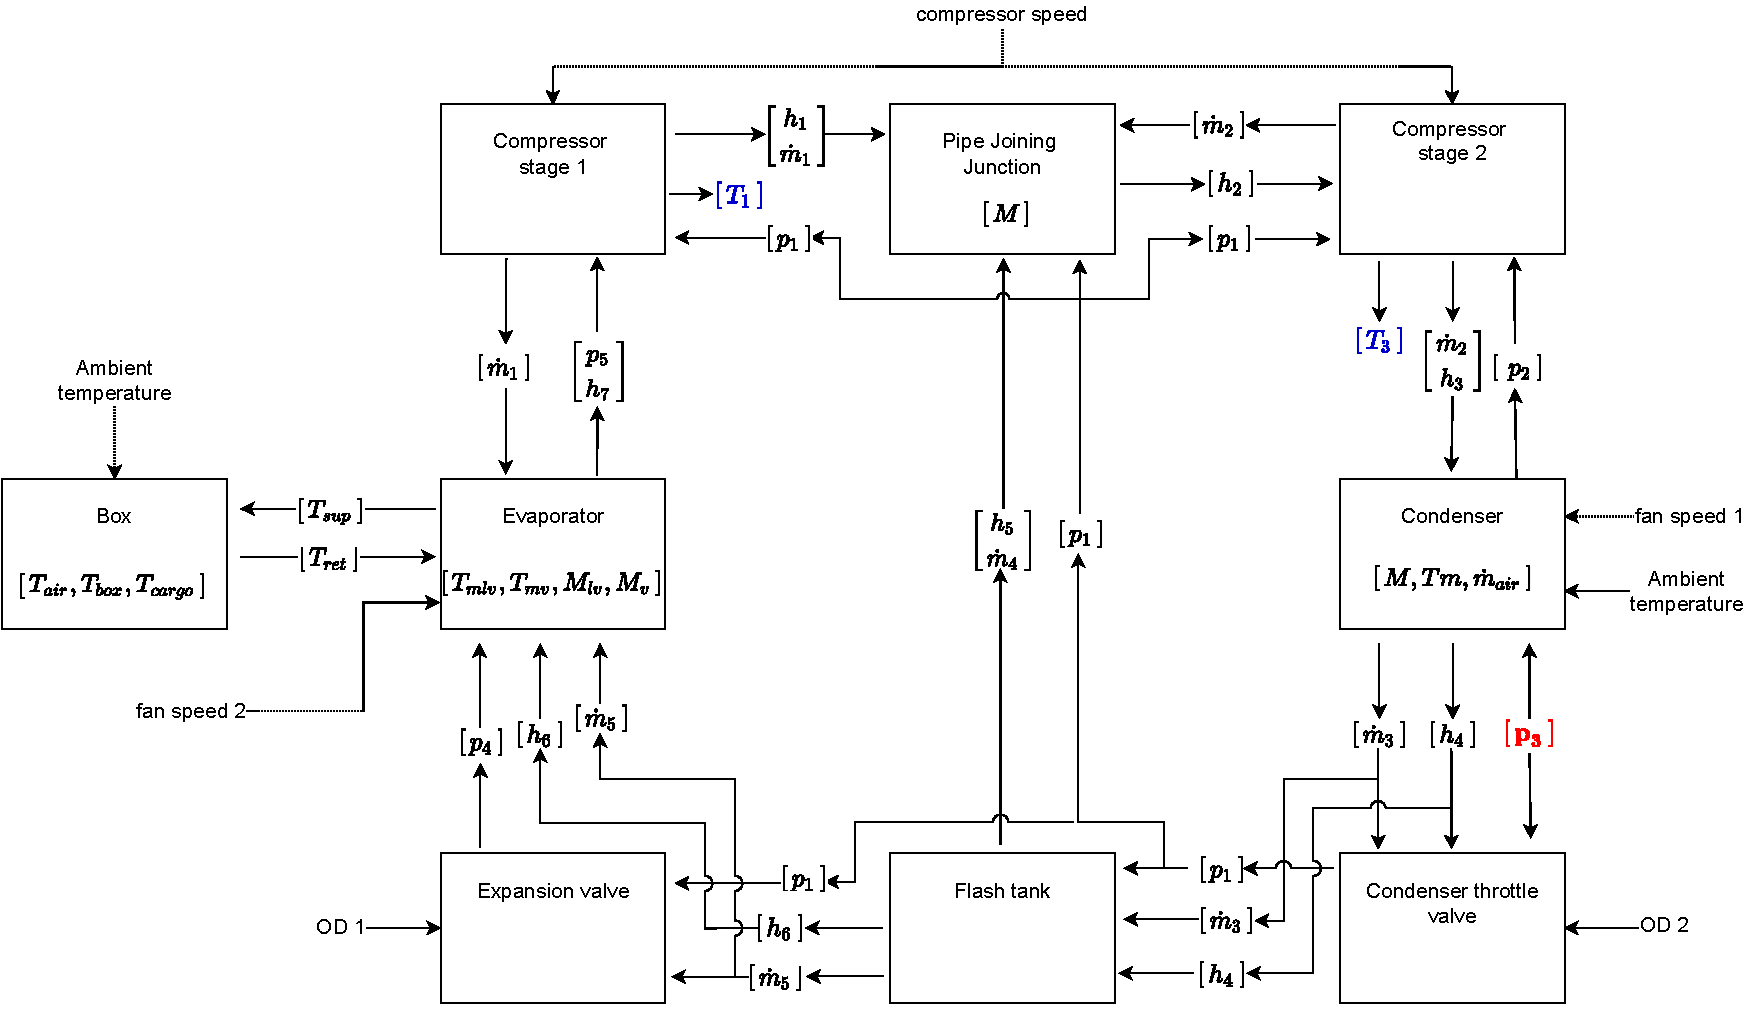
\includegraphics[width=1\textwidth]{Graphics/Block_Diagram_inout.pdf}
	\caption{Block diagram of input/output relationship of interface variables}
	\label{fig:Block_diagram_inout_valvePres}
\end{figure} 
 
 
